% Mid-evaluation deck following the prescribed 3-slide format (Phase 1 work only):
%   1) Problem Statement (group, name + roll no, novelty, contributions)
%   2) Architecture image only, no explanations
%   3) Results and findings in tabular format
\documentclass[aspectratio=141,10pt]{beamer}

\usepackage[T1]{fontenc}
\usepackage{booktabs}
\usepackage{array}
\usepackage{adjustbox}
\usepackage{tikz}
\usetikzlibrary{arrows.meta,positioning,fit,backgrounds}

\definecolor{body}{HTML}{555555}
\definecolor{accent}{HTML}{2A78D6}
\definecolor{boxblue}{HTML}{E8F1FC}
\definecolor{boxorange}{HTML}{FDEEE7}
\definecolor{lineorange}{HTML}{EB6834}
\definecolor{boxgreen}{HTML}{E7F6EF}
\definecolor{linegreen}{HTML}{1BAF7A}

\setbeamertemplate{navigation symbols}{}
\setbeamertemplate{footline}{}
\setbeamercolor{frametitle}{fg=black}
\setbeamercolor{normal text}{fg=body}
\setbeamercolor{itemize item}{fg=body}
\setbeamercolor{itemize subitem}{fg=body}
\setbeamercolor{enumerate item}{fg=body}
\setbeamertemplate{itemize items}{--}
\setbeamertemplate{itemize subitem}{--}
\setbeamerfont{frametitle}{size=\Large}
\setbeamertemplate{frametitle}{\vspace{6pt}\insertframetitle}

\newcommand{\nQuestions}{64,535}
\newcommand{\nCells}{65}
\newcommand{\nQuestionsRun}{64,478}
\newcommand{\gpuHours}{71}
\newcommand{\nCompared}{29}
\newcommand{\nWithinFive}{12}
\newcommand{\nWithinTen}{20}
\newcommand{\medianAbsDelta}{6.0}
\newcommand{\llamaSCemptyOneK}{25.2}
\newcommand{\llamaSCrtwZero}{205}
\newcommand{\llamaSCwtrZero}{51}
\newcommand{\llamaSCfirstZero}{94.4}
\newcommand{\mistralSCrtwZero}{188}
\newcommand{\mistralSCwtrZero}{29}
\newcommand{\mistralSCfirstZero}{95.6}
\newcommand{\posAccAthree}{60}
\newcommand{\posAccDthree}{43}
\newcommand{\posAccAlong}{42}
\newcommand{\posAccDlong}{23}
\newcommand{\posPickDthree}{14}
\newcommand{\posPickDlong}{8}
\newcommand{\llamaRagRefusalAll}{19.1}

\graphicspath{{figures/}}

\begin{document}

%===============================================================================
% Slide 1 - Problem Statement
%===============================================================================
\begin{frame}
\begin{center}{\color{black}\LARGE Problem Statement}\end{center}
\vspace{2pt}
{\small\itshape LLM assistants forget user preferences stated earlier in a conversation (PrefEval, ICLR 2025): accuracy collapses as
unrelated context grows. Project: a trained preference-detection classifier + preference memory + modern retrieval.
Mid-term covers Phase 1.\par}
\vspace{6pt}
\small
\begin{enumerate}
  \setlength{\itemsep}{4pt}
  \item[1)] \textbf{Group Name:} Individual project
  \item[2)] \textbf{Team Name, Roll no:} Krishna Jhanwar, 12341250
  \item[3)] \textbf{Novelty:}
  \begin{itemize}\setlength{\itemsep}{1pt}\footnotesize
    \item \textbf{Overall idea:} a small \emph{trained} classifier detects preference-stating turns and writes them to a structured
          memory (grows with the number of preferences, not turns), combined with a modern retriever (bge / e5, replacing 2021 SimCSE)
    \item \textbf{Phase 1 (done):} PrefEval's Bedrock-only evaluation rebuilt to run fully locally (Ollama, one 12\,GB GPU)
          with the original prompts unchanged: resumable, logged, reproducible
    \item \textbf{Phase 1:} baselines reproduced on two of the paper's models (Llama-3-8B, Mistral-7B): 5 methods,
          explicit + implicit-choice, 0.2k--23k tokens, \nQuestions{} questions; new implicit classification baselines
    \item \textbf{Phase 1:} found and fixed 3 prompt-formatting issues and 2 defects in the released retrieval data; new analyses
          (self-critique overturning answers, position bias at long context, RAG refusals)
  \end{itemize}
  \item[4)] \textbf{Contributions:}
  \begin{itemize}\setlength{\itemsep}{1pt}\footnotesize
    \item[] \textbf{Member 1} --- Krishna Jhanwar (12341250): project design (all phases); Phase 1: local evaluation pipeline,
            debugging of prompt and data issues, all baseline runs ($\approx$\gpuHours{} GPU-hours), aggregation, analysis and reporting
  \end{itemize}
\end{enumerate}
\end{frame}

%===============================================================================
% Slide 2 - Architecture image only (Phase 1 system)
%===============================================================================
\begin{frame}
\frametitle{Architecture}
\centering\hyphenpenalty=10000\exhyphenpenalty=10000
\vspace{8pt}
\begin{adjustbox}{max width=\linewidth, max totalheight=0.86\textheight}
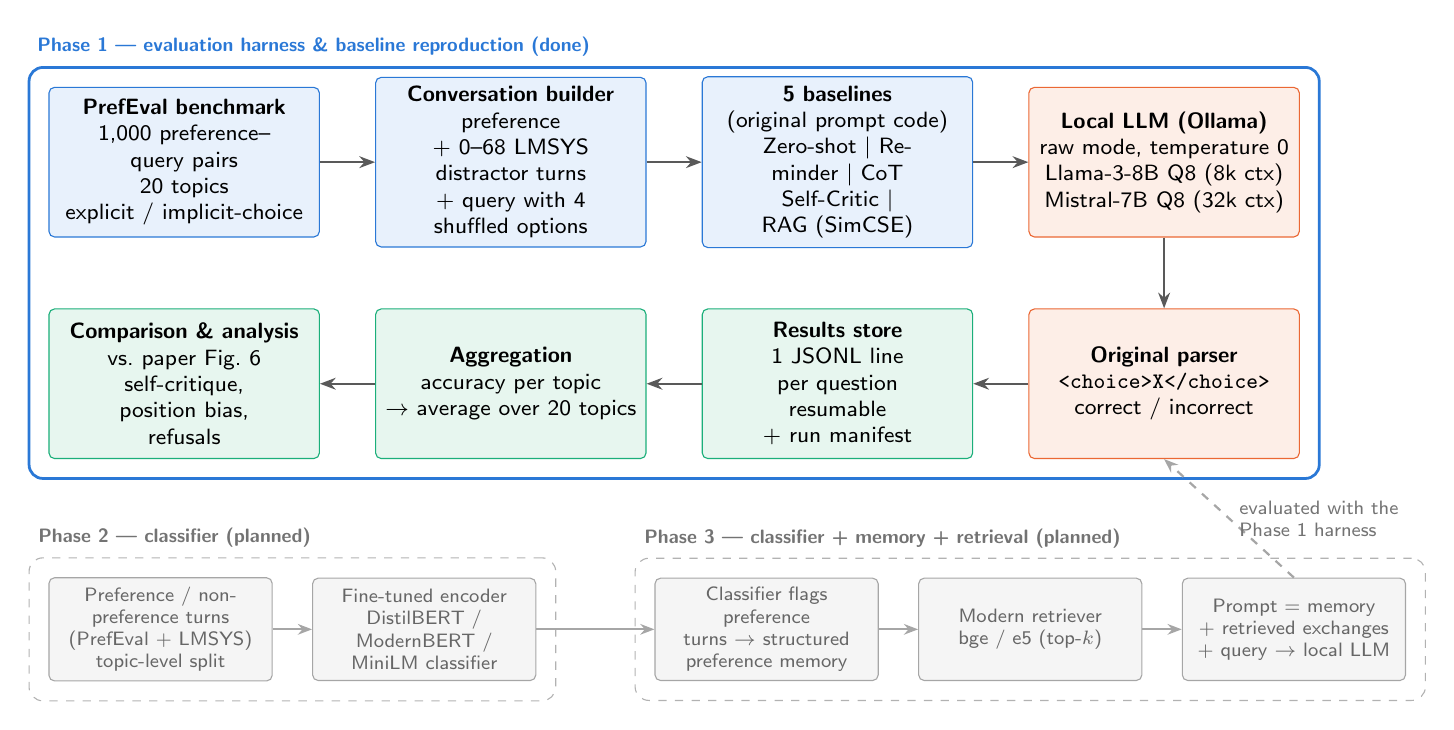
\begin{tikzpicture}[font=\sffamily\footnotesize, node distance=0.9cm and 0.7cm,
  b/.style={draw=accent, fill=boxblue, rounded corners=2pt, align=center, minimum height=1.9cm, text width=3.2cm},
  o/.style={draw=lineorange, fill=boxorange, rounded corners=2pt, align=center, minimum height=1.9cm, text width=3.2cm},
  g/.style={draw=linegreen, fill=boxgreen, rounded corners=2pt, align=center, minimum height=1.9cm, text width=3.2cm},
  p/.style={draw=black!35, fill=black!4, text=black!60, rounded corners=2pt, align=center, minimum height=1.3cm,
            text width=2.6cm, font=\sffamily\scriptsize},
  a/.style={-{Stealth[length=2mm]}, thick, color=black!65},
  pa/.style={-{Stealth[length=1.8mm]}, thick, color=black!35},
  lane/.style={rounded corners=5pt, inner sep=7pt},
  lab/.style={anchor=south west, font=\sffamily\scriptsize\bfseries}]

% ---------------- Phase 1 (done): evaluation harness + baselines
\node[b] (bench) {\textbf{PrefEval benchmark}\\1,000 preference--query pairs\\20 topics\\explicit / implicit-choice};
\node[b, right=of bench] (conv) {\textbf{Conversation builder}\\preference\\+ 0--68 LMSYS distractor turns\\+ query with 4 shuffled options};
\node[b, right=of conv] (meth) {\textbf{5 baselines}\\(original prompt code)\\Zero-shot \textbar{} Reminder \textbar{} CoT\\Self-Critic \textbar{} RAG (SimCSE)};
\node[o, right=of meth] (llm) {\textbf{Local LLM (Ollama)}\\raw mode, temperature 0\\Llama-3-8B Q8 (8k ctx)\\Mistral-7B Q8 (32k ctx)};
\node[o, below=of llm] (parse) {\textbf{Original parser}\\\texttt{<choice>X</choice>}\\correct / incorrect};
\node[g, left=of parse] (store) {\textbf{Results store}\\1 JSONL line per question\\resumable\\+ run manifest};
\node[g, left=of store] (agg) {\textbf{Aggregation}\\accuracy per topic\\$\rightarrow$ average over 20 topics};
\node[g, left=of agg] (cmp) {\textbf{Comparison \& analysis}\\vs.\ paper Fig.\ 6\\self-critique, position bias,\\refusals};
\draw[a] (bench)--(conv); \draw[a] (conv)--(meth); \draw[a] (meth)--(llm);
\draw[a] (llm)--(parse); \draw[a] (parse)--(store); \draw[a] (store)--(agg); \draw[a] (agg)--(cmp);

% ---------------- Phase 2 and 3 (planned), compact and greyed
\node[p, below=1.5cm of cmp.south west, anchor=north west] (p2a) {Preference / non-preference turns\\(PrefEval + LMSYS)\\topic-level split};
\node[p, right=0.5cm of p2a] (p2b) {Fine-tuned encoder\\DistilBERT / ModernBERT /\\MiniLM classifier};
\node[p, right=1.5cm of p2b] (p3a) {Classifier flags preference\\turns $\rightarrow$ structured\\preference memory};
\node[p, right=0.5cm of p3a] (p3b) {Modern retriever\\bge / e5 (top-$k$)};
\node[p, right=0.5cm of p3b] (p3c) {Prompt = memory\\+ retrieved exchanges\\+ query $\rightarrow$ local LLM};
\draw[pa] (p2a)--(p2b); \draw[pa] (p2b)--(p3a); \draw[pa] (p3a)--(p3b); \draw[pa] (p3b)--(p3c);
\draw[pa, dashed] (p3c.north) -- node[right, font=\sffamily\scriptsize, text=black!55, align=left]{evaluated with the\\Phase 1 harness} (parse.south);

\begin{scope}[on background layer]
\node[lane, draw=accent, line width=1pt, fill=white, fit=(bench)(llm)(parse)(cmp)] (L1) {};
\node[lane, draw=black!30, dashed, fit=(p2a)(p2b)] (L2) {};
\node[lane, draw=black!30, dashed, fit=(p3a)(p3c)] (L3) {};
\end{scope}
\node[lab, text=accent] at (L1.north west) {Phase 1 --- evaluation harness \& baseline reproduction (done)};
\node[lab, text=black!55] at (L2.north west) {Phase 2 --- classifier (planned)};
\node[lab, text=black!55] at (L3.north west) {Phase 3 --- classifier + memory + retrieval (planned)};
\end{tikzpicture}
\end{adjustbox}
\end{frame}

%===============================================================================
% Slide 3 - Results and findings in tabular format (+ figure)
%===============================================================================
\begin{frame}
\frametitle{Results and Findings in Tabular Format}
\centering
\vspace{-2pt}
{\scriptsize Explicit preference: classification accuracy (\%), averaged over 20 topics. Paper (left) vs.\ our reproduction (right)\par}
\vspace{2pt}
\resizebox{\linewidth}{!}{\begin{tabular}{llcccccc@{\hspace{10pt}}cccccc}
\toprule
 & & \multicolumn{6}{c}{\textbf{Paper} (Fig.\ 6, Bedrock)} & \multicolumn{6}{c}{\textbf{Ours} (local, Ollama Q8)} \\
\cmidrule(lr){3-8}\cmidrule(lr){9-14}
Model & Method & 0.2k & 1k & 3k & 10k & 16k & 23k & 0.2k & 1k & 3k & 10k & 16k & 23k \\
\midrule
Llama-3-8B & Zero-shot & 85 & 55 & 42 & -- & -- & -- & 94.2 & 52.7 & 43.3 & -- & -- & -- \\
 & Reminder & 94 & 80 & 59 & -- & -- & -- & 97.4 & 78.0 & 59.4 & -- & -- & -- \\
 & CoT & 83 & 67 & 50 & -- & -- & -- & 93.7 & 78.0 & 63.9 & -- & -- & -- \\
 & Self-Critic & 79 & 73 & 62 & -- & -- & -- & 78.8 & 50.1 & 46.7 & -- & -- & -- \\
 & RAG & -- & 87 & 80 & -- & -- & -- & -- & 88.6 & 74.8 & -- & -- & -- \\
\midrule
Mistral-7B & Zero-shot & 87 & 66 & 57 & 50 & 42 & 47 & 95.5 & 61.5 & 55.5 & 42.5 & 37.1 & 37.6 \\
 & Reminder & 95 & 85 & 75 & 63 & 56 & 56 & 96.2 & 78.9 & 71.3 & 56.7 & 43.9 & 46.9 \\
 & CoT & 90 & 79 & 73 & 69 & 56 & 62 & 88.0 & 74.9 & 67.0 & -- & -- & -- \\
 & Self-Critic & 75 & 65 & 58 & 51 & 52 & 48 & 79.8 & 67.0 & 61.0 & -- & -- & -- \\
 & RAG & -- & 87 & 86 & 81 & 80 & 75 & -- & 81.0 & 75.7 & 64.6 & 59.0 & 53.7 \\
\bottomrule
\end{tabular}
}\\[1pt]
{\tiny -- = not available: Llama-3-8B has an 8k context limit (as in the paper); RAG is undefined at 0.2k; our CoT and Self-Critic were run up to 3k only.\par}

\vspace{5pt}
\begin{minipage}[t]{0.36\linewidth}\centering
{\scriptsize Explicit vs.\ implicit (choice) at 3k tokens (\%)\par}\vspace{2pt}
\resizebox{\linewidth}{!}{\begin{tabular}{lcccc}
\toprule
 & \multicolumn{2}{c}{Llama-3-8B} & \multicolumn{2}{c}{Mistral-7B} \\
\cmidrule(lr){2-3}\cmidrule(lr){4-5}
Method & Explicit & Implicit & Explicit & Implicit \\
\midrule
Zero-shot & 43.3 & 46.0 & 55.5 & 47.5 \\
Reminder & 59.4 & 60.2 & 71.3 & 63.1 \\
CoT & 63.9 & 61.7 & 67.0 & 59.5 \\
Self-Critic & 46.7 & 38.7 & 61.0 & 50.9 \\
RAG & 74.8 & 73.7 & 75.7 & 64.0 \\
\bottomrule
\end{tabular}
}
\end{minipage}\hfill
\begin{minipage}[t]{0.61\linewidth}\centering
{\scriptsize Key findings\par}\vspace{2pt}
\resizebox{\linewidth}{!}{%
\begin{tabular}{ll}
\toprule
Finding & Evidence \\
\midrule
Baselines reproduced locally & \nWithinFive/\nCompared{} cells within 5 pts; \nWithinTen/\nCompared{} within 10 \\
Accuracy decays with context & Mistral Zero-shot 95.5 $\rightarrow$ 37.6 (0.2k $\rightarrow$ 23k) \\
RAG most robust at long context & 23k: RAG 53.7 vs.\ Zero-shot 37.6 \\
Self-critique overturns answers & Llama, 0.2k: \llamaSCrtwZero{} right$\rightarrow$wrong vs.\ \llamaSCwtrZero{} wrong$\rightarrow$right \\
Long context $\rightarrow$ position prior & 23k: accuracy \posAccAlong{} (answer A) vs.\ \posAccDlong{} (answer D) \\
Implicit preferences harder & Mistral: 7--15 pts below explicit \\
Retrieval triggers refusals & Llama RAG, 3k: \llamaRagRefusalAll\% without a valid choice \\
\bottomrule
\end{tabular}}
\end{minipage}
\end{frame}

\end{document}
